\chapter{Execução}
\section{Arquitetura geral}
A arquitetura geral do software foi projetada com base nos objetivos expostos no início do documento. Inicialmente foi feito o desenvolvimento dos casos de uso e do diagrama de blocos, de forma a visualizar o funcionamento do sistema como um todo. O resultado está descrito nas seções a seguir.

\subsection{Software da estação-base e do placa TS-7260}

\begin{enumerate}[topsep=0pt, partopsep=0pt, itemsep=0pt]
  \item Visualização de mapa 2D na interface gráfica segundo os dados lidos dos sensores do robô. Representado pelo caso de uso: \textbf{``Mostrar mapa - UC\arabic{enumi}''}.
  \item Gravação do mapa em um arquivo no disco rígido. Representado pelo caso de uso: \textbf{``Salvar mapa - UC\arabic{enumi}''}. 
  \item Leitura do mapa de um arquivo do disco rígido. Representado pelo caso de uso: \textbf{``Carregar mapa - UC\arabic{enumi}''}.
  \item Leitura de informações dos sensores do robô. Representado pelo caso de uso: \textbf{``Ler amostras dos sensores - UC\arabic{enumi}''}.
  \item Visualização de imagens da \textit{webcam} do robô. Representado pelo caso de uso: \textbf{``Visualizar imagens da câmera - UC\arabic{enumi}''}.
  \item Alteração pelo usuário da velocidade das rodas do robô. Representado pelo caso de uso: \textbf{``Alterar velocidade das rodas - UC\arabic{enumi}''}.
  \item Solicitação de estabelecimento de conexão com o robô. \textbf{``Estabelecer conexão - UC\arabic{enumi}''}.
%  \item Inclusão de novos obstáculos e suas posições lidos do robô. Representado pelo caso de uso: \textbf{``Mostrar posição dos novos obstáculos detectados na tela - UC\arabic{enumi}''}.
  \item Consulta à documentação do robô pelo usuário. Representado pelo caso de uso: \textbf{``Consultar documentação do robô - UC\arabic{enumi}''}.
\end{enumerate}

Foram produzidos três Diagramas de Casos de Uso (Figuras \ref{fig:diagrama_caso_uso_estacao_base}, \ref{fig:diagrama_caso_uso_linux_embarcado} e \ref{fig:diagrama_caso_uso_placa_embarcada}) com base nos casos de uso apresentados. O primeiro diagrama representa o \textit{software} da estação base, e o segundo e o terceiro representam o sistema embarcado (TS-7260 e placa de baixo nível, respectivamente).

\begin{figure}[H]
  \centering
  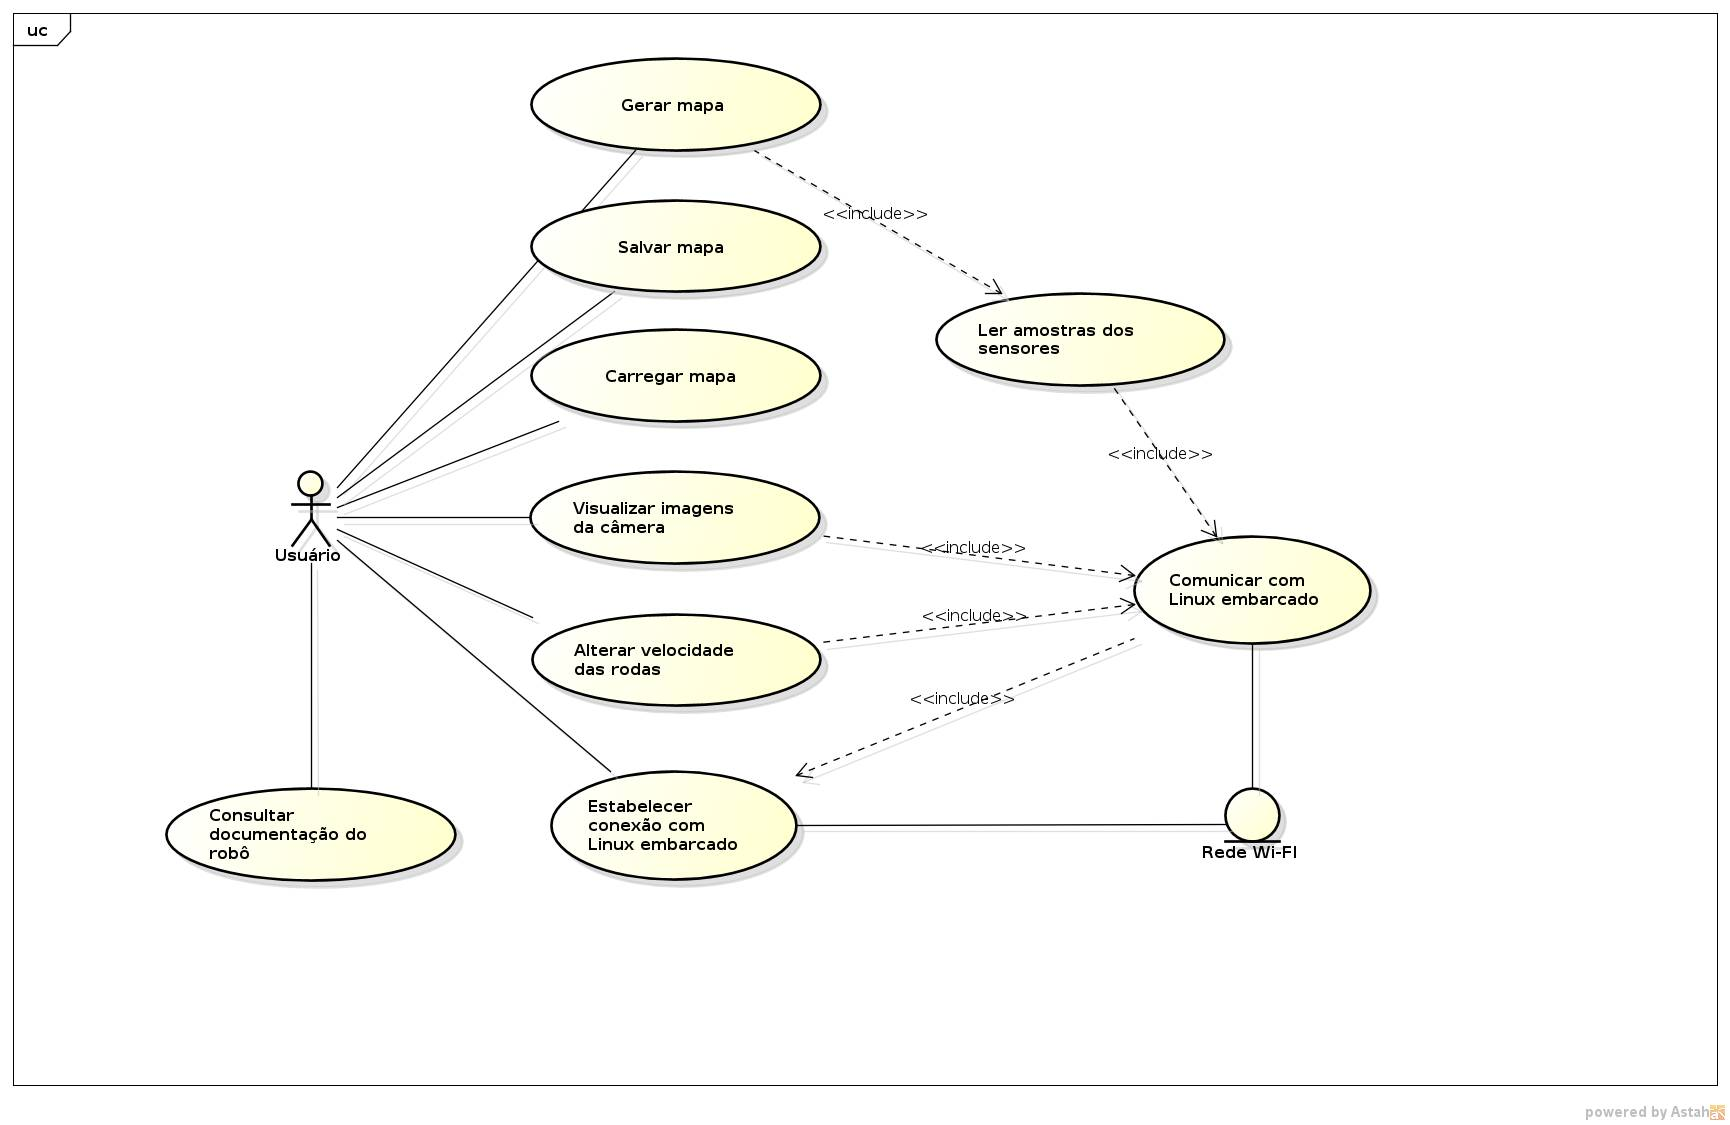
\includegraphics[width=\textwidth, keepaspectratio]{./figuras/estacaoBase/usecase_estacao_base.jpg}
  \caption{Diagrama de casos de uso do \textit{software} da estação base.}
  \label{fig:diagrama_caso_uso_estacao_base}
\end{figure}

\begin{figure}[H]
  \centering
  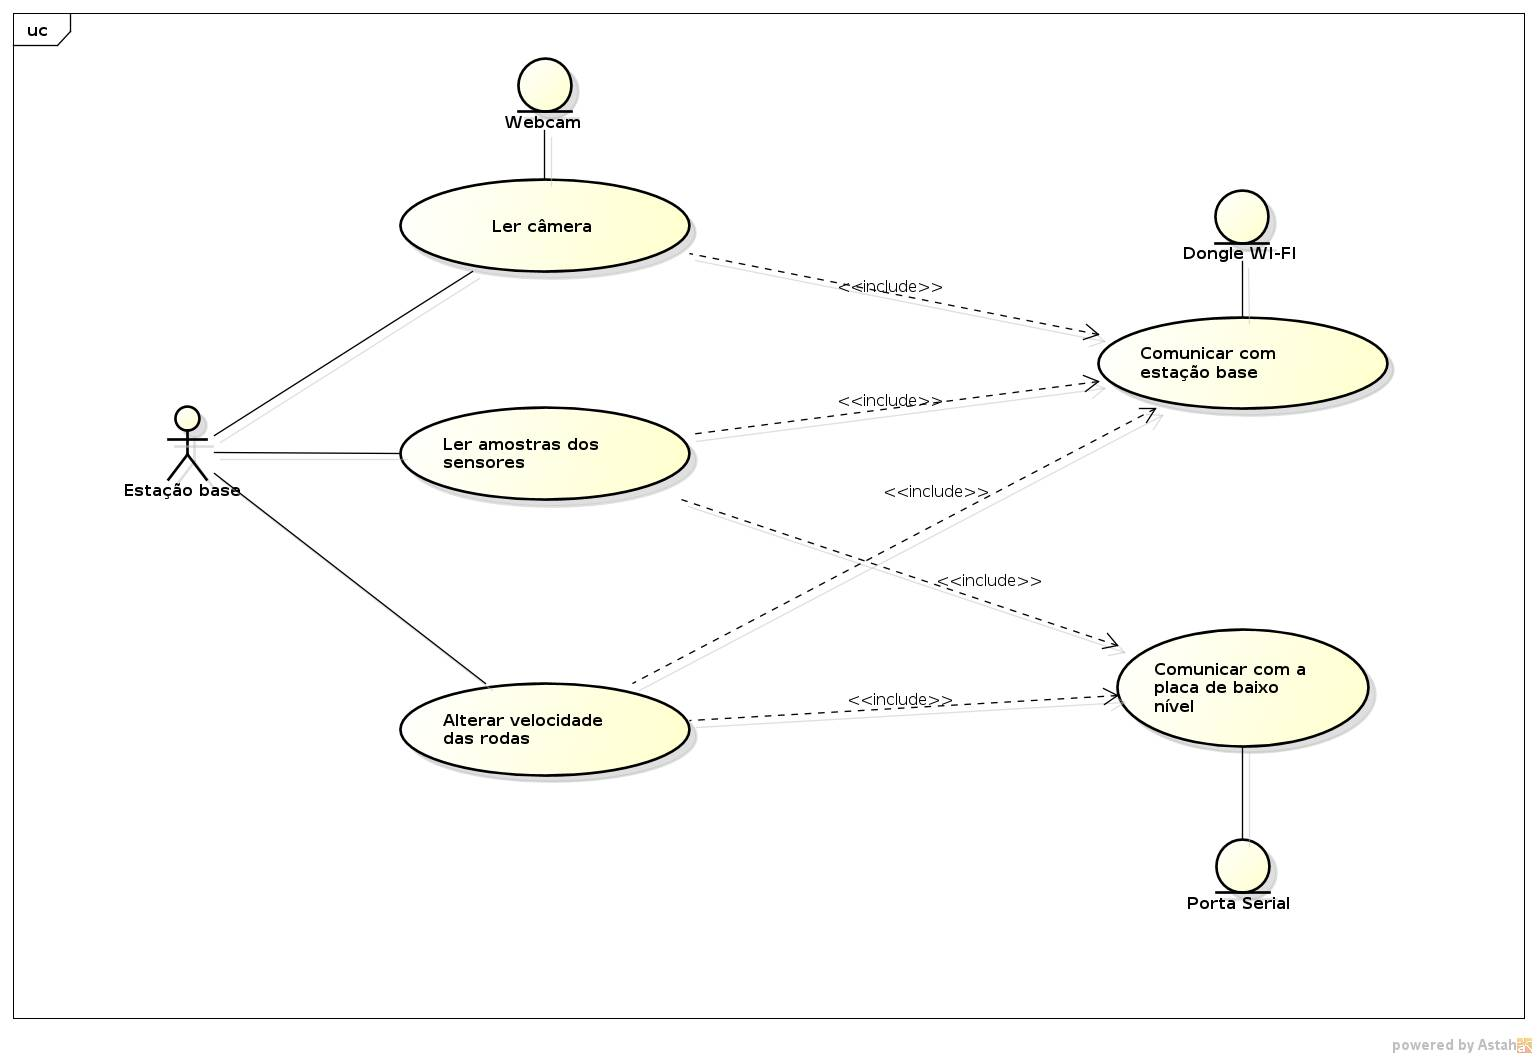
\includegraphics[width=\textwidth, keepaspectratio]{./figuras/sistEmbarcado/usecase_linux_embarcado.jpg}
  \caption{Diagrama de casos de uso do \textit{software} para a placa TS-7260.}
  \label{fig:diagrama_caso_uso_linux_embarcado}
\end{figure}

\begin{figure}[H]
  \centering
  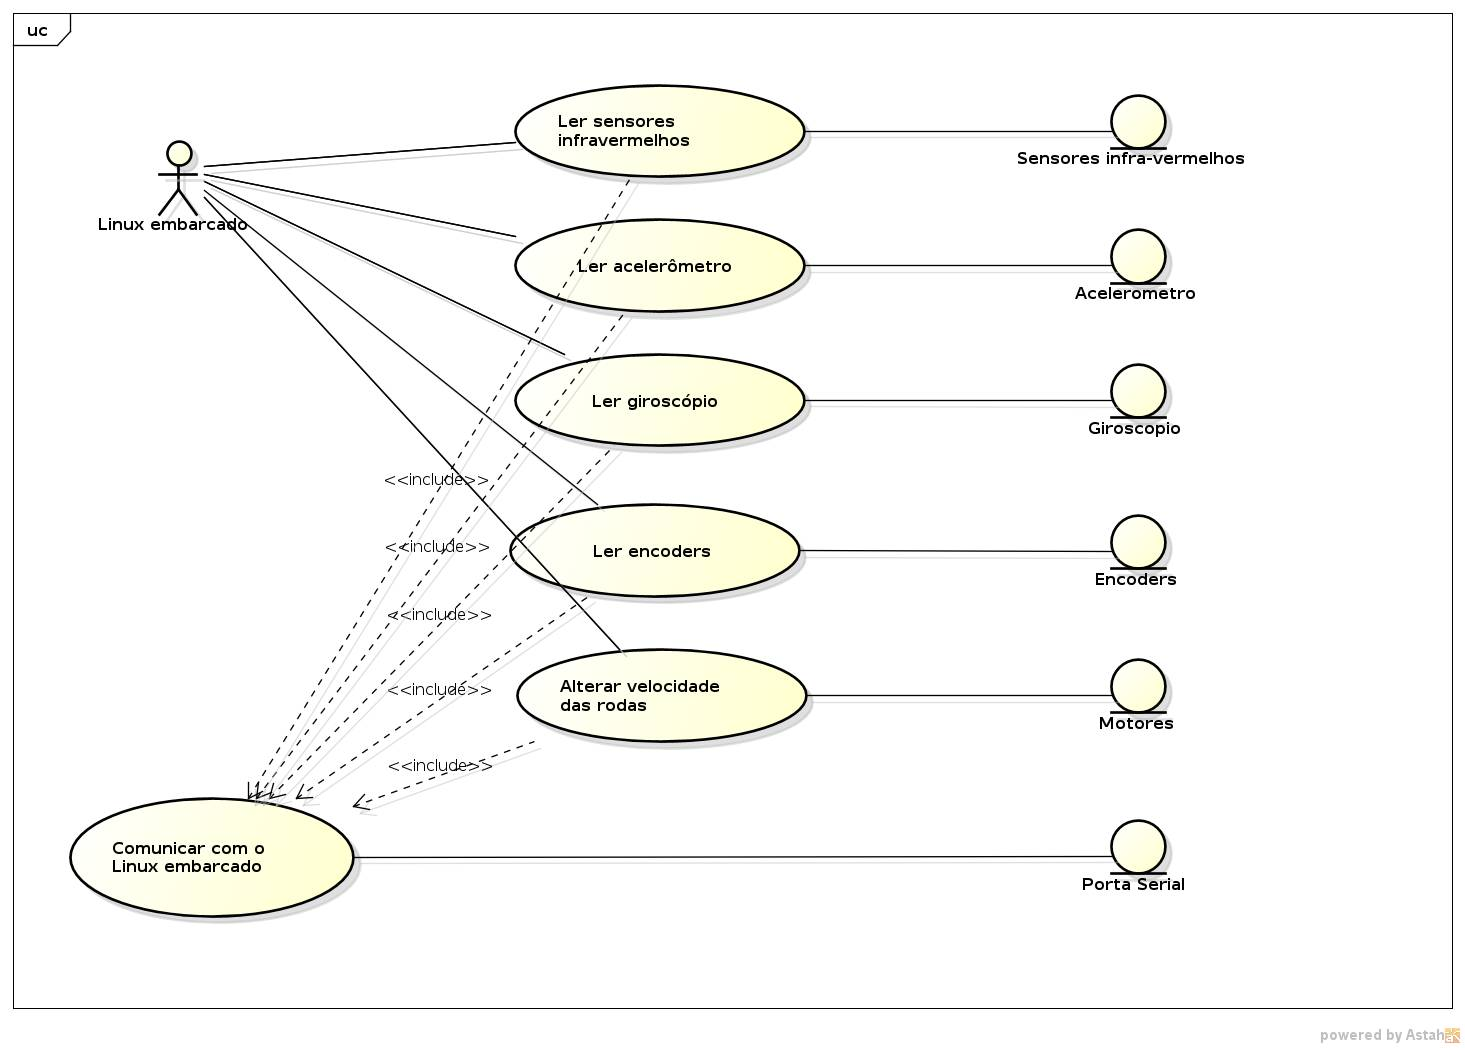
\includegraphics[width=\textwidth, keepaspectratio]{./figuras/sistEmbarcado/usecase_placa_baixo_nivel.jpg}
  \caption{Diagrama de casos de uso do \textit{software} para a placa de baixo nível.}
  \label{fig:diagrama_caso_uso_placa_embarcada}
\end{figure}

\subsection{Hardware}

Na figura \ref{fig:diagrama_blocos_hardware} mostra-se o diagrama de blocos do sistema embarcado e suas conexões com o restante do robô. A seguir está também uma descrição para cada um dos blocos da placa de circuito impresso do sistema embarcado.

\begin{figure}[H]
  \centering
  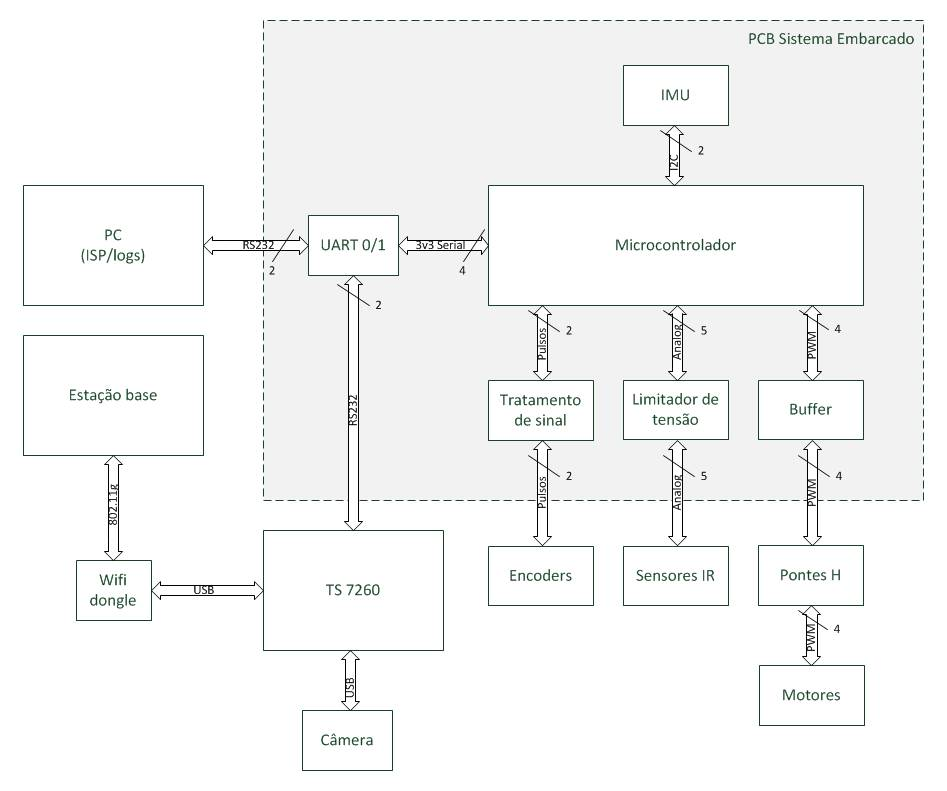
\includegraphics[width=\textwidth]{./figuras/hardware/diagrama_blocos_hardware.jpg}
  \caption{Diagrama de blocos do hardware}
  \label{fig:diagrama_blocos_hardware}
\end{figure}


\begin{enumerate}[topsep=0pt, partopsep=0pt, itemsep=0pt]
    \item Microcontrolador: Este bloco fará a leitura dos sensores: encoders, infra-vermelhos, acelerômetro e giroscópios. Além disso possui a implementação do protocolo de comunicação para interação com o linux embarcado da placa TS-7260.
    \item UART 0/1: Responsável por ajustar os níveis de tensão para comunicação serial no padrão RS-232 com a placa TS-7260.
    \item Buffer: Responsável por fornecer corrente e elevar os níveis de tensão de saída do microcontrolador de 3,3V para 5,0V. Esse buffer é conectado às pontes H já existentes no robô.
    \item IMU (Inertial Measurement Unit): possui o acelerômetro e o giroscópio e se comunicará com o microcontrolador por meio do protocolo I2C.
    \item Limitador de tensão: Necessário pois os sinais de saída dos sensores de infravermelho que já existem no robô não estão limitados em 5V, podendo a saída ultrapassar 5,0V e danificar o microcontrolador. 
    \item Tratamento de sinal: Composto por um filtro RC passa baixas e um Schmitt trigger para remover qualquer falha que possa ocorrer na geração dos pulsos no encoder.
\end{enumerate}

\section{Estação-base}
\subsection{Diagrama de classes da estação base}

A Figura \ref{fig:diagrama_classes_estacao_base} mostra o diagrama de classes da estação base.
\begin{figure}[H]
  \centering
  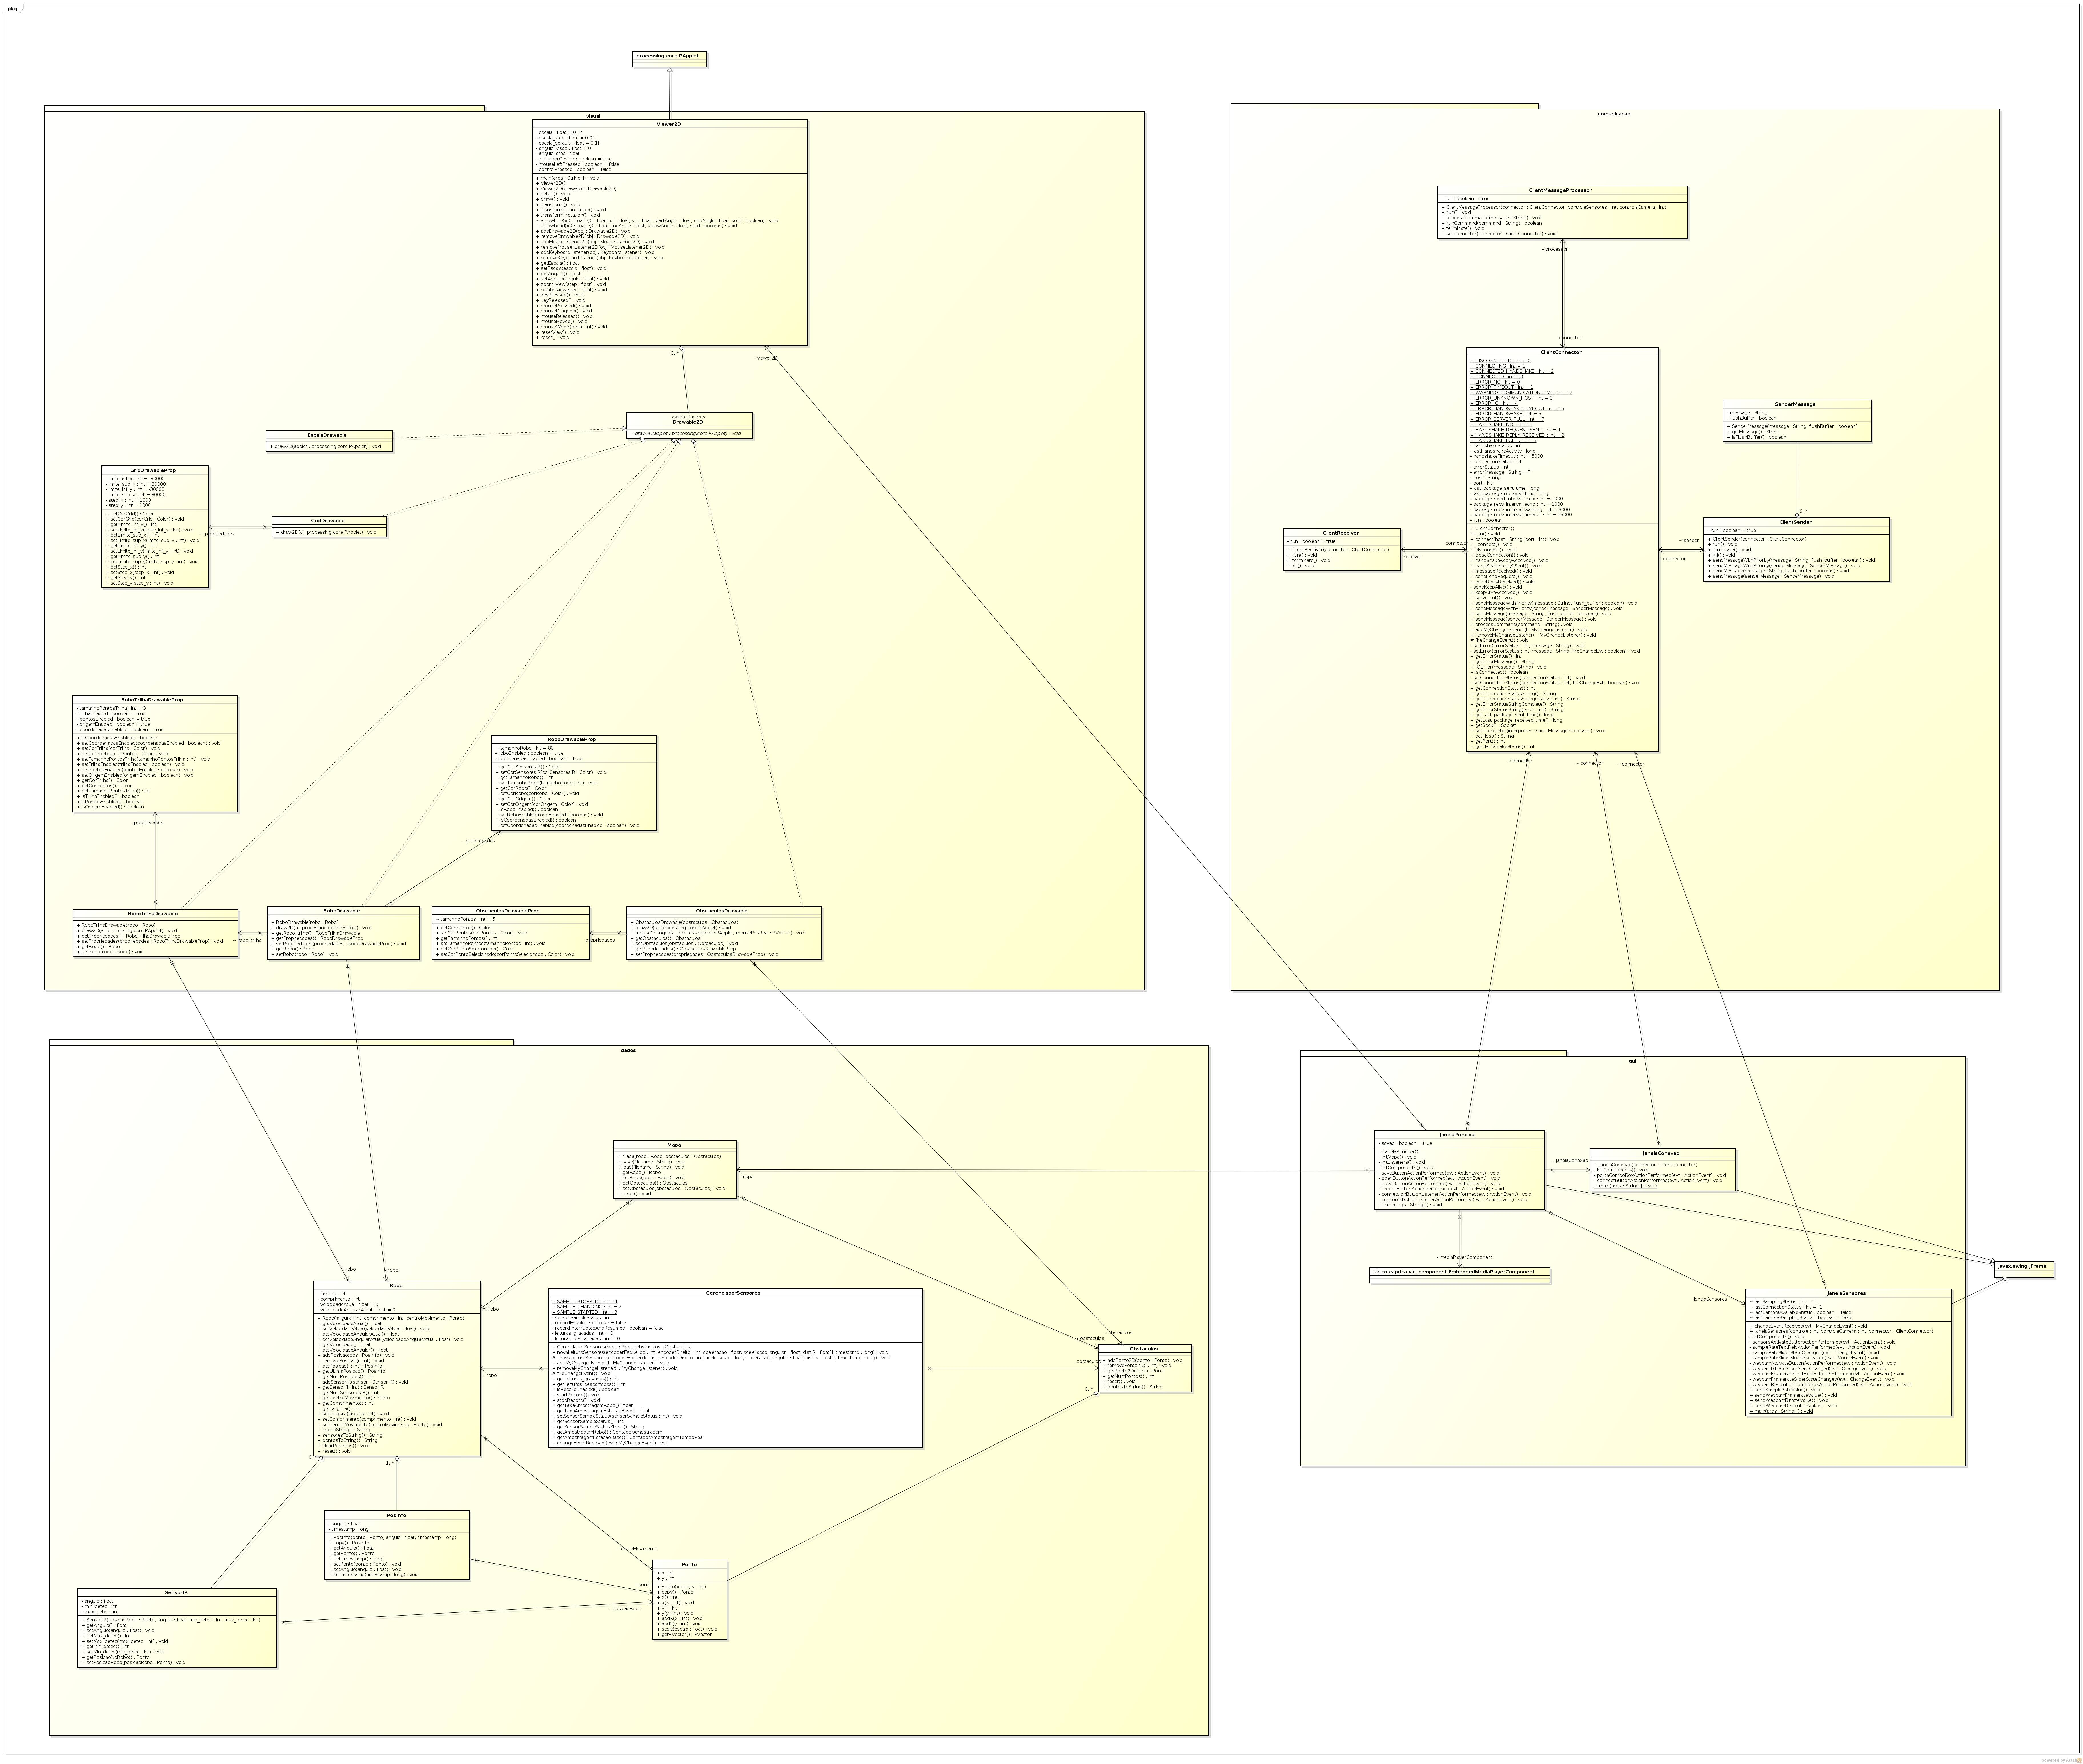
\includegraphics[width=\textwidth]{./figuras/estacaoBase/class_estacaoBase.jpg}
  \caption{Diagrama de classes da estação base}
  \label{fig:diagrama_classes_estacao_base}
\end{figure}

\subsubsection{Descrição das classes da estação base}
%O software da estação base do robô foi dividido em cinco pacotes:  visual, controle, comunicação, controle.robo e interface gráfica. Estes serão descritos com suas respectivas classes na Tabela \ref{tab:pacote_visual}.
O \textit{software} da estação base do robô foi dividido em cinco pacotes:  \textit{visual}, \textit{dados}, \textit{comunicacao}, e \textit{gui}. A seguir há uma descrição de cada pacote e das suas respectivas classes.


\subsubsection{Pacote \textit{visual}}

Este pacote consiste de toda a parte visual da estação base e conta com as seguintes classes: Viewer2D, Drawable2D, EscalaDrawable, RoboDrawable, RoboTrilhaDrawable, ObstaculosDrawable, EscalaDrawableProp, RoboDrawableProp, RoboTrilhaDrawableProp e ObstaculosDrawableProp. Na Tabela \ref{tab:pacote_visual} estão descritas as classes deste pacote.


\begin{table}[H]
  \centering
  \caption{Pacote \textit{visual}}
  \begin{tabular}{p{6cm}p{8cm}}
    \toprule
    \textbf{Classe} & \textbf{Descrição} \\
    \midrule
    Viewer2D & Responsável por exibir os objetos Drawable2D. Possui recursos de pan, zoom e rotate.   \\ \hline
    Drawable2D & Representa genericamente objetos 2D que podem ser desenhados em um Viewer2D. \\ \hline
    EscalaDrawable & Responsável por desenhar uma escala gráfica no mapa. \\ \hline
    RoboDrawable & Responsável por desenhar o robô no mapa. \\ \hline
    RoboTrilhaDrawable & Responsável por desenhar a trilha percorrida pelo robô no mapa. \\ \hline
    ObstaculosDrawable & Responsável por desenhar os pontos de cada obstáculo no mapa. \\ \hline
    EscalaDrawableProp & Contém as propriedades visuais de desenho da escala. \\ \hline
    RoboDrawableProp & Contém as propriedades visuais de desenho do robô \\ \hline
    RoboTrilhaDrawableProp & Contém as propriedades visuais de desenho da trilha do robô. \\ \hline
    ObstaculosDrawableProp & Contém as propriedades visuais de desenho dos obstáculos. \\
    \bottomrule
  \end{tabular}%
  \label{tab:pacote_visual}%
\end{table}%

\subsubsection{Pacote \textit{dados}}

Este pacote consiste de toda a parte da estação base que processa e armazena as informações essenciais do robô e do mapa. Conta com as seguintes classes: Mapa, Obstaculos, Robo, ControleSensores, Posinfo, SensorIR e Ponto. Na Tabela \ref{tab:pacote_controle} estão descritas as classes deste pacote.

\begin{table}[H]
  \centering
  \caption{Pacote \textit{dados}}
  \begin{tabular}{p{6cm}p{8cm}}
    \toprule
    \textbf{Classe} & \textbf{Descrição} \\ 
    \midrule
    Mapa  & Responsável por representar o mapa. Armazena as informações essenciais do robô e dos obstáculos detectados. \\ \hline
    Obstaculos & Responsável por conter os obstáculos detectados pelo robô. \\ \hline
    Robo  & Responsável por representar o robô, este contêm largura, comprimento e centro de movimento (ponto central entre as duas rodas). \\ \hline
    GerenciadorSensores & Responsável por atualizar a posição do robô e dos pontos que representam os obstáculos, de acordo com as leituras feitas pelos sensores. \\ \hline
    Posinfo & Responsável por conter as informações de uma posição do robô. \\ \hline
    SensorIR & Responsável por representar um sensor IR do robô. \\ \hline 
    Ponto & Representa um ponto de cordenadas cartesianas (x,y). \\ \hline
    GerenciadorCamera & Responsável por gerenciar o status da câmera e o recebimento de imagens. \\ 
    \bottomrule
  \end{tabular}%
  \label{tab:pacote_controle}%
\end{table}%

\subsubsection{Pacote \textit{comunicacao}}
\label{subsec:pacote_comunicacao}

%Este pacote consiste em toda a parte de comunicação da estação base com o robô e conta com as seguintes classes: ClientCommandInterpreter, ClientConnection, ClientReceiver, ClientSender, ServerCommandInterpreter, ServerListener, ServerSender, ServerReceiver e Message. Na Tabela \ref{tab:pacote_comunicacao} estão descritas as classe deste pacote.
Este pacote consiste em toda a parte de comunicação da estação base com o robô e conta com as seguintes classes: ClientMessageProcessor ClientConnection, ClientReceiver, ClientSender e Message. Na Tabela \ref{tab:pacote_comunicacao} estão descritas as classes deste pacote.

É importante ressaltar que o protocolo TCP requer obrigatoriamente a especificação de um cliente e de um servidor para estabelecimento de uma conexão. Nas implementações desse protocolo em diversas linguagens (como Java e C++) existem tipos de \textit{socket} distintos para cliente e servidor. Na criação de um \textit{socket} de servidor, há obrigatoriamente a atribuição de uma porta de escuta, na qual o servidor aguarda que um cliente efetue uma requisição de conexão. Não é possível, ao menos nas implementações atuais do TCP, estabelecer conexão entre dois \textit{sockets} de cliente ou entre dois \textit{sockets} de servidor. Como neste projeto, o robô proverá serviços à estação base (envio de imagens da câmera, envio de leituras de sensores, além de prover a possibilidade de comando dos motores) o robô foi escolhido como servidor e a estação base como cliente. Enfatiza-se que o paradigma cliente-servidor não implica de forma alguma que a comunicação seja unidirecional. Pelo contrário, o envio de pacotes 
pode ser feito bidirecionalmente após uma conexão TCP ser estabelecida, sem nenhuma restrição quanto a isso.

\begin{table}[H]
  \centering
  \caption{Pacote \textit{comunicacao}}
  \begin{tabular}{p{6cm}p{8cm}}
    \toprule
    \textbf{Classe} & \textbf{Descrição} \\ 
    \midrule
    ClientMessageProcessor & Thread responsável pelo processamento de mensagens recebidas de um host de conexão. \\ \hline
    ClientConnector & Thread responsável por efetuar a gerência da conexão do cliente (estação base) com o servidor (robô). \\ \hline
    ClientReceiver & Thread responsável por receber mensagens de um host de uma conexão. \\ \hline
    ClientSender & Thread responsável por enviar mensagens ao host de uma conexão. \\ \hline
%    ServerCommandInterpreter & Responsável pela interpretação dos comandos do servidor. Os comandos recebidos são inseridos em uma fila, de modo a serem posteriormente executados pela thread. \\ \hline
%    Server & Responsável gerenciar o servidor (robô). \\ \hline
%    ServerListener & Responsável por escutar as novas conexões de clientes. \\ \hline
%    ServerSender & Responsável por enviar mensagens ao host de uma conexão. \\ \hline
%    ServerReceiver & Responsável por receber mensagens de um host de uma conexão. \\ \hline
    SenderMessage & Contém uma mensagem que pode ser enviada por um Sender. \\ \hline
    \bottomrule
  \end{tabular}%
  \label{tab:pacote_comunicacao}%
\end{table}%

\subsubsection{Pacote \textit{gui}}

Este pacote consiste em toda a interface gráfica do sistema e conta com as seguintes classes: JanelaConexao, JanelaPrincipal e JanelaSensores. Na Tabela \ref{tab:pacote_interface_grafica} estão descritas as classes deste pacote.

\begin{table}[H]
  \centering
  \caption{Pacote \textit{gui}}
  \begin{tabular}{p{6cm}p{8cm}}
    \toprule
    \textbf{Classe} & \textbf{Descrição} \\ 
    \midrule
    JanelaConexao & Janela com as informações e configurações da conexão com o Bellator. \\ \hline
    JanelaPrincipal & Janela principal da interface gráfica da estação base. \\ \hline
    JanelaSensores & Janela de configuração dos sensores. \\ 
    \bottomrule
  \end{tabular}%
  \label{tab:pacote_interface_grafica}%
\end{table}%

% \section{Fluxo de dados}
% 
% A Figura \ref{fig:diagrama_fluxo_dados} mostra o diagrama de fluxo de dados.
% 
% \begin{figure}[H]
%   \centering
%   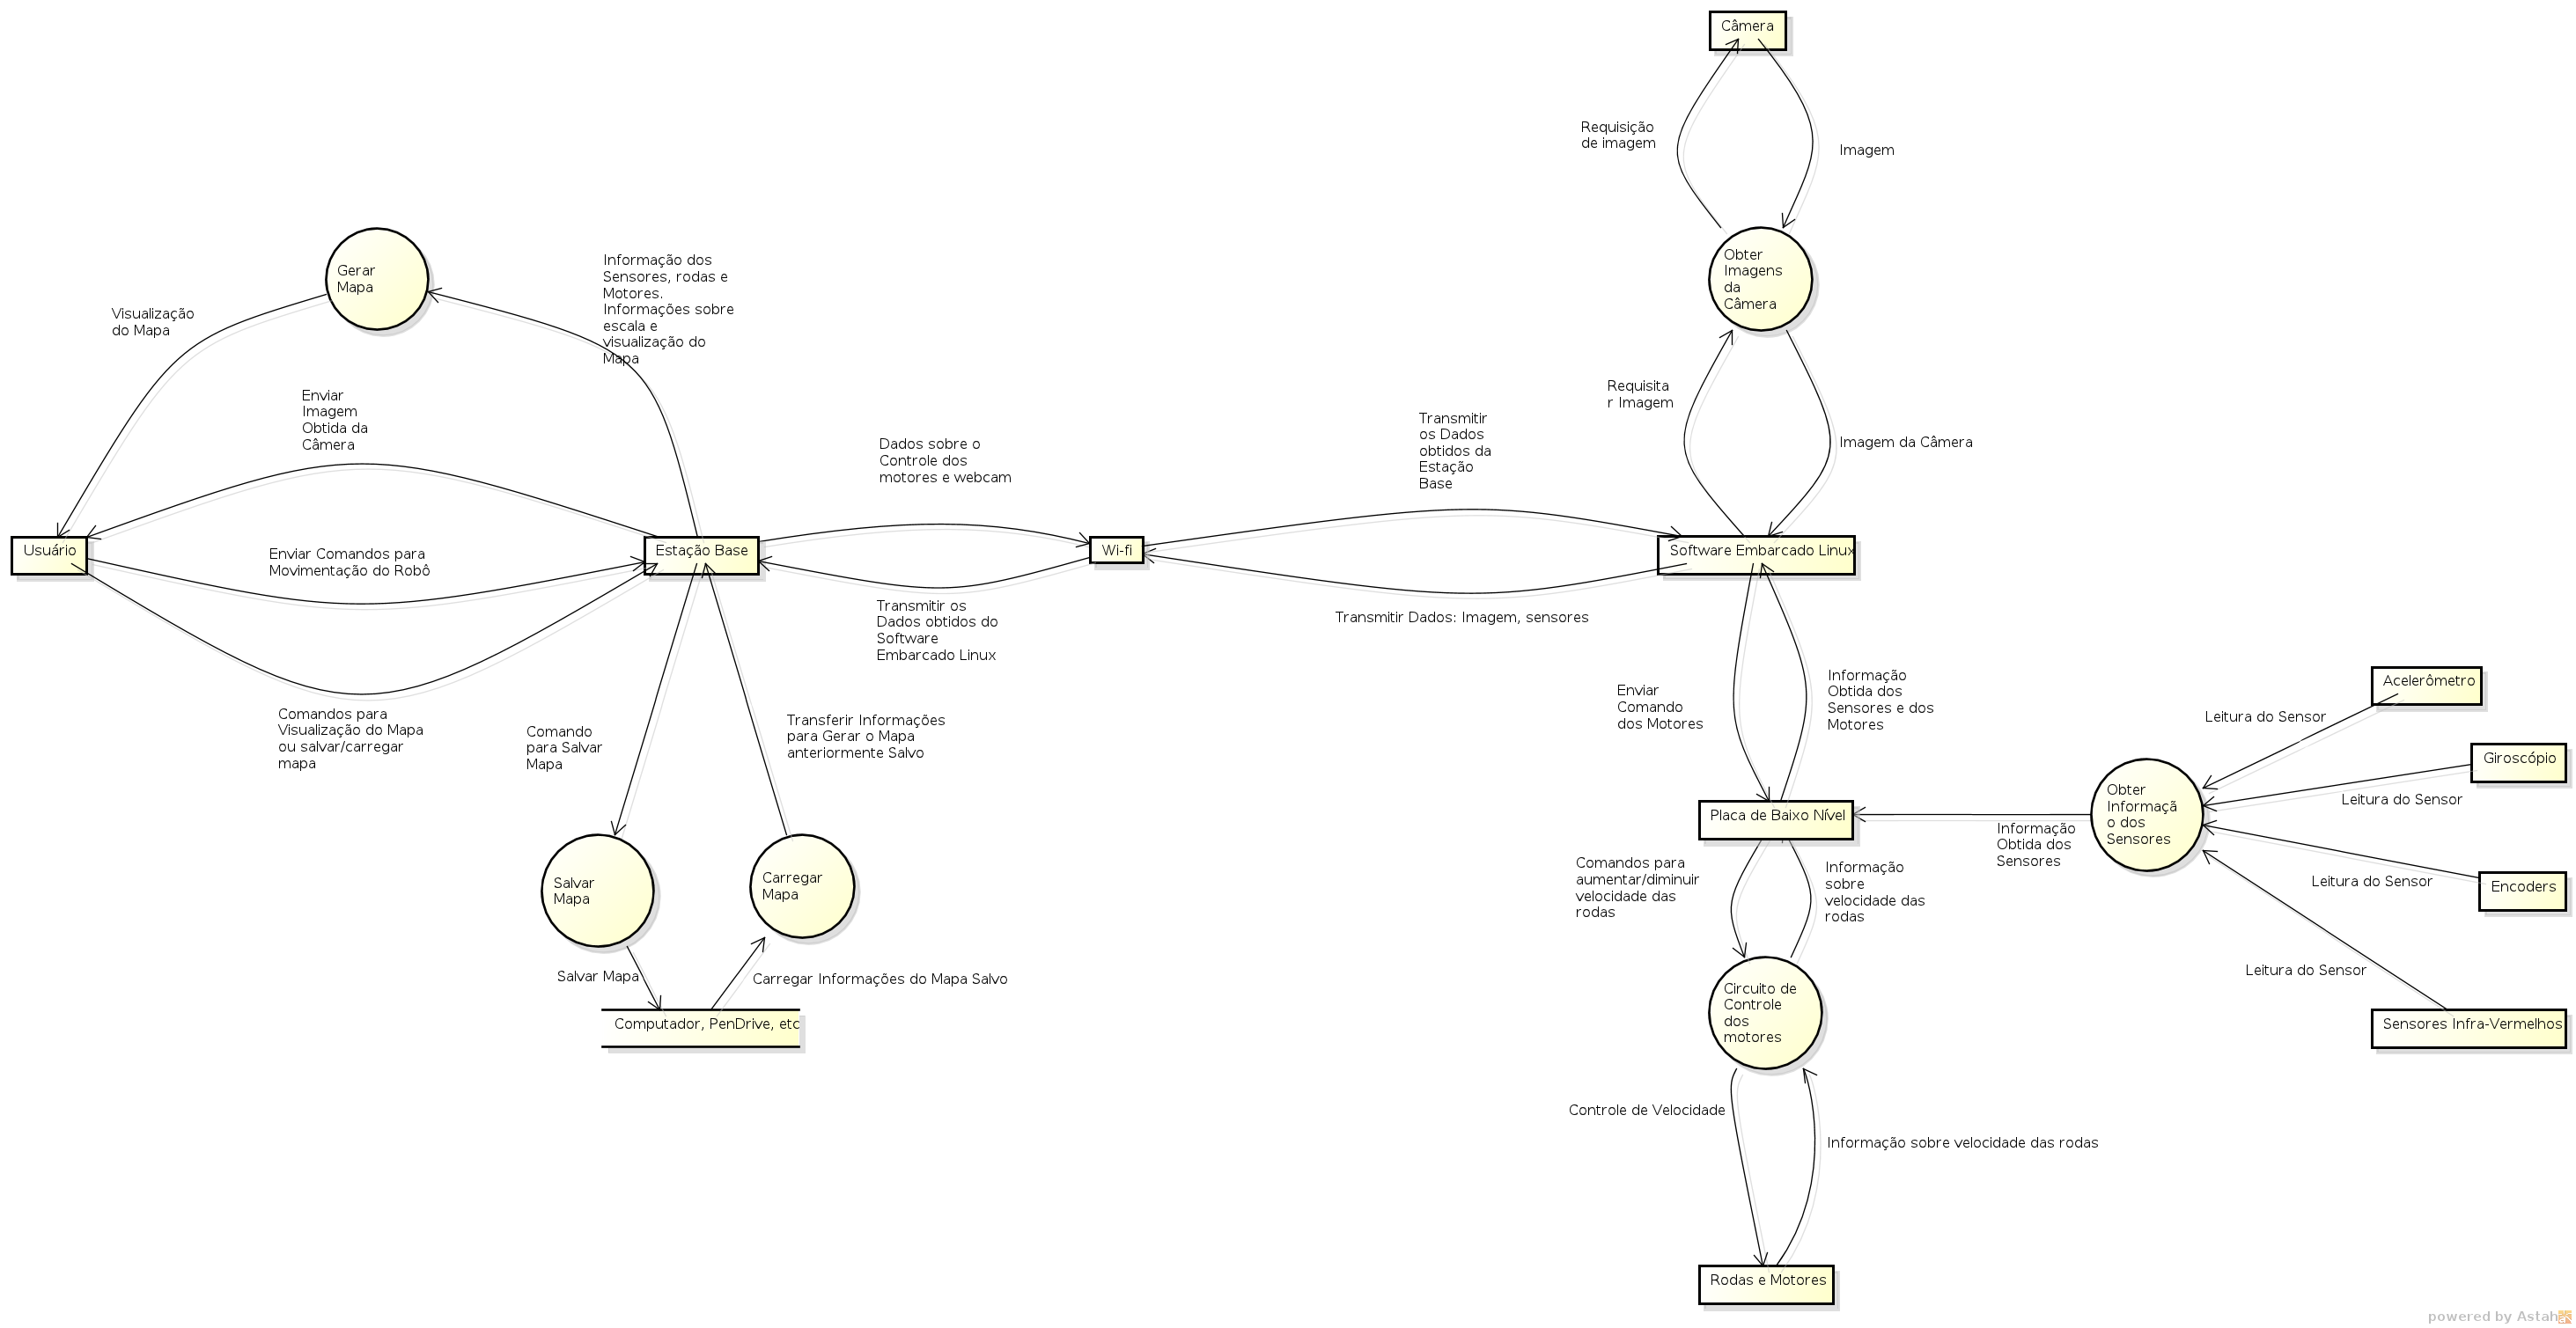
\includegraphics[width=\textwidth, keepaspectratio]{./figuras/diagrama_fluxo_dados.jpg}
%   \caption{Diagrama de fluxo de dados.}
%   \label{fig:diagrama_fluxo_dados}
% \end{figure}

% \section{Diagrama de estados}
% As Figuras \ref{fig:diagrama_estados_estacao_base} e \label{fig:diagrama_estados_sistema_embarcado} mostram os diagramas de estados do sistema.
% 
% \begin{figure}[H]
%   \centering
%   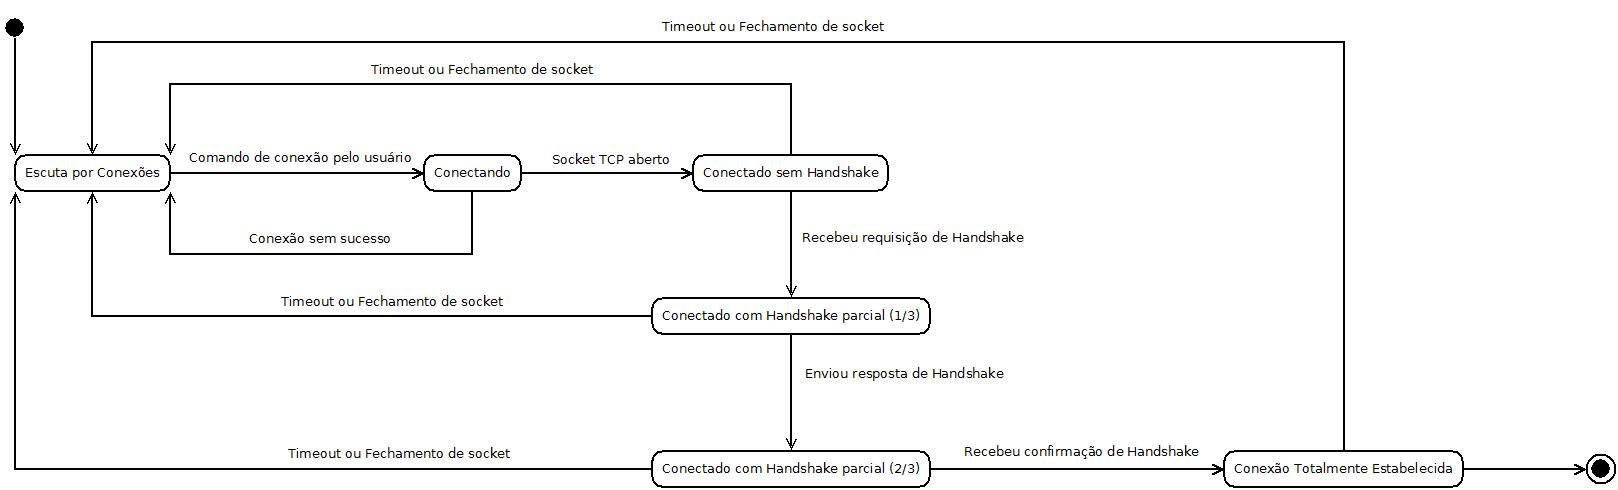
\includegraphics[width=\textwidth, keepaspectratio]{./figuras/diagrama_estados_estacao_base.jpeg}
%   \caption{Diagrama de estados para a estação base.}
%   \label{fig:diagrama_estados_estacao_base}
% \end{figure}
% 
% \begin{figure}[H]
%   \centering
%   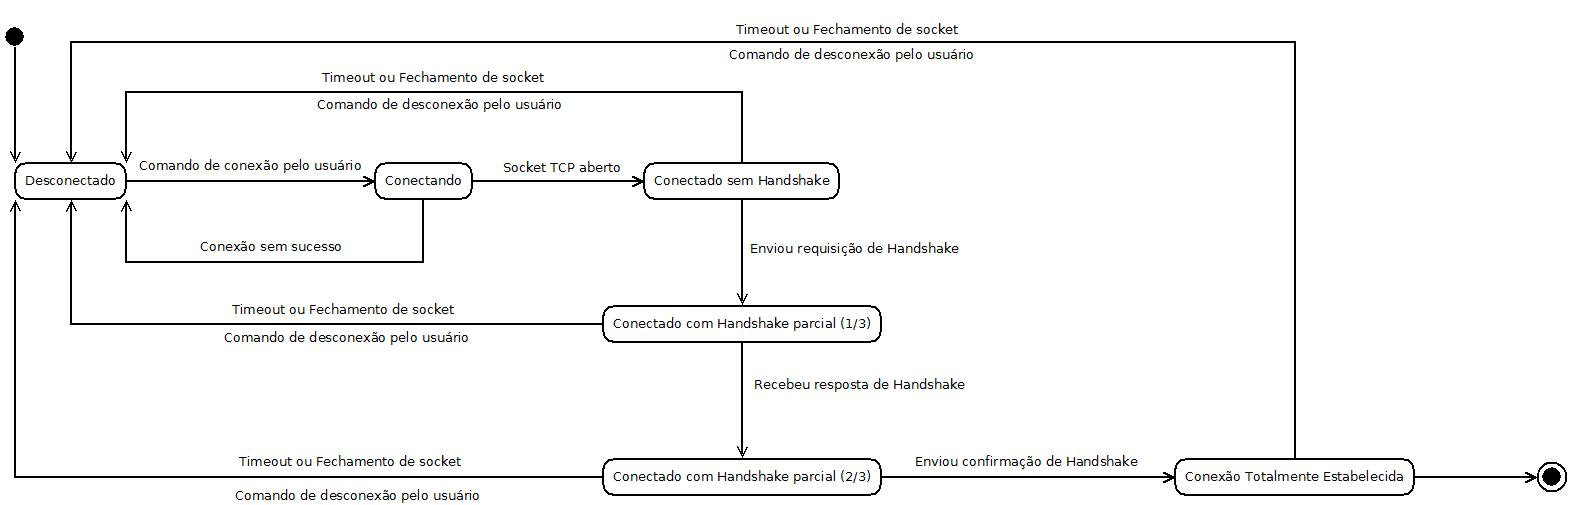
\includegraphics[width=\textwidth, keepaspectratio]{./figuras/diagrama_estados_sistema_embarcado.jpeg}
%   \caption{Diagrama de estados para o sistema embarcado.}
%   \label{fig:diagrama_estados_sistema_embarcado}
% \end{figure}

\section{Sistema de comunicação}
\subsection{Codificação das mensagens}
\label{sec:codificacao_mensagens}

\begin{itemize}
  \item Mensagens do TS-7260 para o LPC2103 (via porta serial)
    	
	\begin{itemize}
		
	  \item \textbf{SYNC (0xA0)}\\
	  Quando o microcontrolador LPC2103 recebe esta mensagem, responde com as leituras mais recentes dos encoders, de cada sensor de distância, do acelerômetro e do giroscópio (enviando uma mensagem SENSORS, explicada abaixo).
	  
	  \item \textbf{ENGINES (0xB0)}\\
	  \textit{(byte) vel\_roda\_esquerda}\\
	  \textit{(byte) vel\_roda\_direita}\\
	  \textit{(byte) CHECKSUM\_H}\\
	  \textit{(byte) CHECKSUM\_L}\\
	  Ao receber este comando, o microcontrolador utiliza os valores para definir o nível de PWM para as rodas do robô. Os valores de velocidade são representados por um byte cada, nos quais o bit mais significativo indica o sentido de rotação da roda (1 para frente e 0 para trás) e os restantes a intensidade do PWM.
	  
	  Os bytes de checksum são utilizados para verificar se não há dados corrompidos. Os bytes da mensagem são somados (módulo 65536) e o resultado é atribuído aos bytes (high e low) de checksum.
	  \end{itemize}
	  
	  \item Mensagens do LPC2103 para a TS-7260 (via porta serial)
	  
	  \begin{itemize}

	  \item \textbf{ENGINES\_ACK (0xB1)}\\
	  \textit{(byte) vel\_roda\_esquerda}\\
	  \textit{(byte) vel\_roda\_direita}\\
	  \textit{(byte) CHECKSUM\_H}\\
	  \textit{(byte) CHECKSUM\_L}\\
	  Esta mensagem deve ser enviada toda vez que um comando de mudança de velocidade (ENGINES) for recebido na placa de baixo nível. A mensagem é usada no Linux embarcado para verificar se o comando foi corretamente recebido. Caso uma confirmação não seja recebida em certo intervalo de tempo, outro comando ENGINES é enviado para a placa de baixo nível.
	 
	  O checksum tem função idêntica ao que já foi explicitado na mensagem ENGINES.
	  
	  \item \textbf{SENSORS (0xC0)}\\
	  \textit{(byte) encoder\_esq\_H}, \textit{(byte) encoder\_esq\_L},\\
	  \textit{(byte) encoder\_dir\_H}, \textit{(byte) encoder\_dir\_L},\\
	  \textit{(byte) IR1}, \textit{(byte) IR2}, \textit{(byte) IR3}, \textit{(byte) IR4}, \textit{(byte) IR5},\\
	  \textit{(byte) AX\_H}, \textit{(byte) AX\_L},\\
	  \textit{(byte) AY\_H}, \textit{(byte) AY\_L},\\
	  \textit{(byte) AZ\_H}, \textit{(byte) AZ\_L},\\
	  \textit{(byte) GX\_H}, \textit{(byte) GX\_L},\\
	  \textit{(byte) GY\_H}, \textit{(byte) GY\_L},\\
	  \textit{(byte) GZ\_H}, \textit{(byte) GZ\_L},\\
	  \textit{(byte) TIMESTAMP\_H}, \textit{(byte) TIMESTAMP\_L}\\
	  \textit{(byte) CHECKSUM\_H}\\
	  \textit{(byte) CHECKSUM\_L}\\
	  Representa a leitura de todos os sensores (encoders, infra-vermelhos, acelerômetro e giroscópio). 
	  
	  Os 4 primeiros bytes são os valores das leituras dos encoders esquerdo e direito (cada um com um byte alto e um baixo). Os valores das leituras dos encoders representam a diferença entre a contagem atual a contagem anterior.
	  
	  Nos próximos 5 bytes, as leituras do sensores ópticos são enviadas em sequência. As distâncias que os sensores ópticos são capazes de mensurar são divididos em valores discretos de 0 a 255 \cite{bellator_2012}. 
	  
	  Após isso, os 12 bytes que se seguem representam as leituras do acelerômetro e do giroscópio. Os bytes que começam com `A' representam a leitura de cada um dos eixos do acelerômetro. Aqueles que começam com `G' representam a leitura de cada um dos eixos do giroscópio.
	  
	  O timestamp (valor alto e baixo) é um contador de 16 bits que é incrementado entre cada amostra e zera automaticamente depois que chega ao valor máximo (65535), usado para determinar o instante em que foi feita a leitura dos dados. Como a amostragem dos sensores na placa de baixo nível será efetuada em intervalos fixos, a informação do contador do timestamp pode ser utilizada para obter informações de tempo de cada amostra.

	  O checksum é tem função idêntica ao que já foi explicitado na mensagem ENGINES.
	  
	  
	\end{itemize}

  \item Mensagens bidirecionais entre estação base e TS-7260 (via WI-Fi):

    \begin{itemize}
      \item \textbf{ECHO\_REQUEST (0x01)}\\
      \textit{(byte) END\_CMD}\\
	Requisição de ping.
      \item \textbf{ECHO\_REPLY (0x02)}\\
      \textit{(byte) END\_CMD}\\
	Resposta de ping.
      \item \textbf{DISCONNECT (0x0F)} \\
	Solicitação de desconexão.
    \end{itemize}

  \item Mensagens da estação base para a TS-7260 (via Wi-Fi):

    \begin{itemize}
      \item \textbf{HANDSHAKE\_REQUEST (0x10)}\\
	Solicitação de handshake.

      \item \textbf{HANDSHAKE\_CONFIRMATION (0x12)}\\
	Confirmação de handshake.

      \item \textbf{SENSORS\_START (0x20)}\\
	Solicitação de início da amostragem dos sensores.

      \item \textbf{SENSORS\_STOP (0x21)}\\
	Solicitação de parada da amostragem dos sensores.

      \item \textbf{SENSORS\_RATE (0x22)} \\
	\textit{(float) Nova taxa de amostragem (comandos SYNC por segundo)}\\
	Solicitação de mudança da taxa de envio de comandos SYNC da TS para a placa de baixo nível.

%       \item \textbf{SENSORS\_STATUS\_REQUEST}\\
%       \textit{(byte) END\_CMD}\\
% 	Requisição de status da amostragem dos sensores. Usado na interface gráfica para atualizar as informações sobre os sensores.

      \item \textbf{WEBCAM\_START (0x30)}\\
	Solicitação de início da amostragem da webcam.

      \item \textbf{WEBCAM\_STOP (0x31)}\\
	Solicitação de parada da amostragem da webcam.

      \item \textbf{WEBCAM\_RATE (0x32)} \\
	\textit{(float) Nova taxa de quadros}\\
	Solicitação de mudança da taxa de quadros da webcam.

      \item \textbf{WEBCAM\_RESOLUTION (0x33)} \\
	\textit{(int) Largura em pixels }\\
	\textit{(int) Altura em pixels}\\
	Solicitação de mudança da resolução da webcam.

%       \item \textbf{WEBCAM\_STATUS\_REQUEST}\\
%       \textit{(byte) END\_CMD}\\
% 	Solicitação de informações sobre status da webcam. Usado na interface gráfica para atualizar as informações sobre a webcam.

      \item \textbf{ENGINES (0xB0)} \\
	 \textit{(float) vel\_roda\_esquerda}\\
	 \textit{(float) vel\_roda\_direita}\\
	Solicitação de mudança da velocidade dos motores. Para cada roda há um valor de -1 até 1, sendo que -1 é a máxima velocidade para trás, 1 a máxima velocidade para frente e 0 é parada da roda.

%       \item \textbf{ENGINES\_STATUS\_REQUEST}\\
%       \textit{(byte) END\_CMD}\\
% 	Solicitação de status dos motores. Usado na interface gráfica para confirmar o recebimento de comandos de movimentação efetuados pelo usuário.

    \end{itemize}

  \item Mensagens da TS-7260 para a estação base (via Wi-Fi):

    \begin{itemize}
      \item \textbf{HANDSHAKE\_REPLY (0x11)}\\
	Resposta de handshake.
	
	 \item \textbf{SENSORS (0xC0)}\\
	  \textit{(byte) encoder1\_H}, \textit{(byte) encoder1\_L},\\
	  \textit{(byte) encoder2\_H}, \textit{(byte) encoder2\_L},\\
	  \textit{(byte) IR1}, \textit{(byte) IR2}, \textit{(byte) IR3}, \textit{(byte) IR4}, \textit{(byte) IR5},\\
	  \textit{(byte) AX\_H}, \textit{(byte) AX\_L},\\
	  \textit{(byte) AY\_H}, \textit{(byte) AY\_L},\\
	  \textit{(byte) AZ\_H}, \textit{(byte) AZ\_L},\\
	  \textit{(byte) GX\_H}, \textit{(byte) GX\_L},\\
	  \textit{(byte) GY\_H}, \textit{(byte) GY\_L},\\
	  \textit{(byte) GZ\_H}, \textit{(byte) GZ\_L},\\
	  \textit{(byte) TIMESTAMP\_H}, \textit{(byte) TIMESTAMP\_L}\\
	  
	  Possui a mesma funcionalidade e parâmetros que a mensagem SENSORS enviada da LPC2103 para a TS-7260, com exceção do timestamp, que é trocado por um timestamp UNIX em milissegundos (que representa o horário absoluto em que a amostra foi obtida na placa de baixo nível). Essa informação de tempo é utilizada pela estação base para efetuar os cálculos de posicionamento do robô.

      \item \textbf{SENSORS\_STATUS (0xC1)} \\
	\textit{(boolean) Status da amostragem [on - off] }\\
	\textit{(float) Taxa de amostragem}\\
	Informações de status dos sensores. Usado na interface gráfica para confirmar o recebimento de comandos de mudança de taxa de amostragem e início/parada da amostragem.

      \item \textbf{WEBCAM\_STATUS (0x34)} \\
% 	\textit{(boolean) Nova taxa de amostragem }\\
	\textit{(float) Taxa de quadros }\\
	\textit{(int) Largura em pixels }\\
	\textit{(int) Altura em pixels }\\
	\textit{(boolean) Status da stream [on - off] }\\
	\textit{(int) Porta da stream}\\
	Informações de status da webcam. Usado na interface gráfica para confirmar o recebimento de comandos relativos à webcam, e para que a estação base tenha conhecimento do status da stream da webcam.
	
      \item \textbf{ENGINES\_STATUS (0xB1)} \\
	\textit{(byte) vel\_roda\_esquerda}\\
	\textit{(byte) vel\_roda\_direita}\\
	Informações sobre as velocidades programadas dos motores. Usado na interface gráfica para confirmar o recebimento de comandos de movimentação efetuados pelo usuário.

	

    \end{itemize}
\end{itemize}


\section{Sistema embarcado}
\subsection{Diagram de classes do sistema embarcado}
A Figura \ref{fig:diagrama_classes_sist_embarcado} mostra o diagrama de classes do sistema embarcado (placa TS-7260).
\begin{figure}[H]
  \centering
  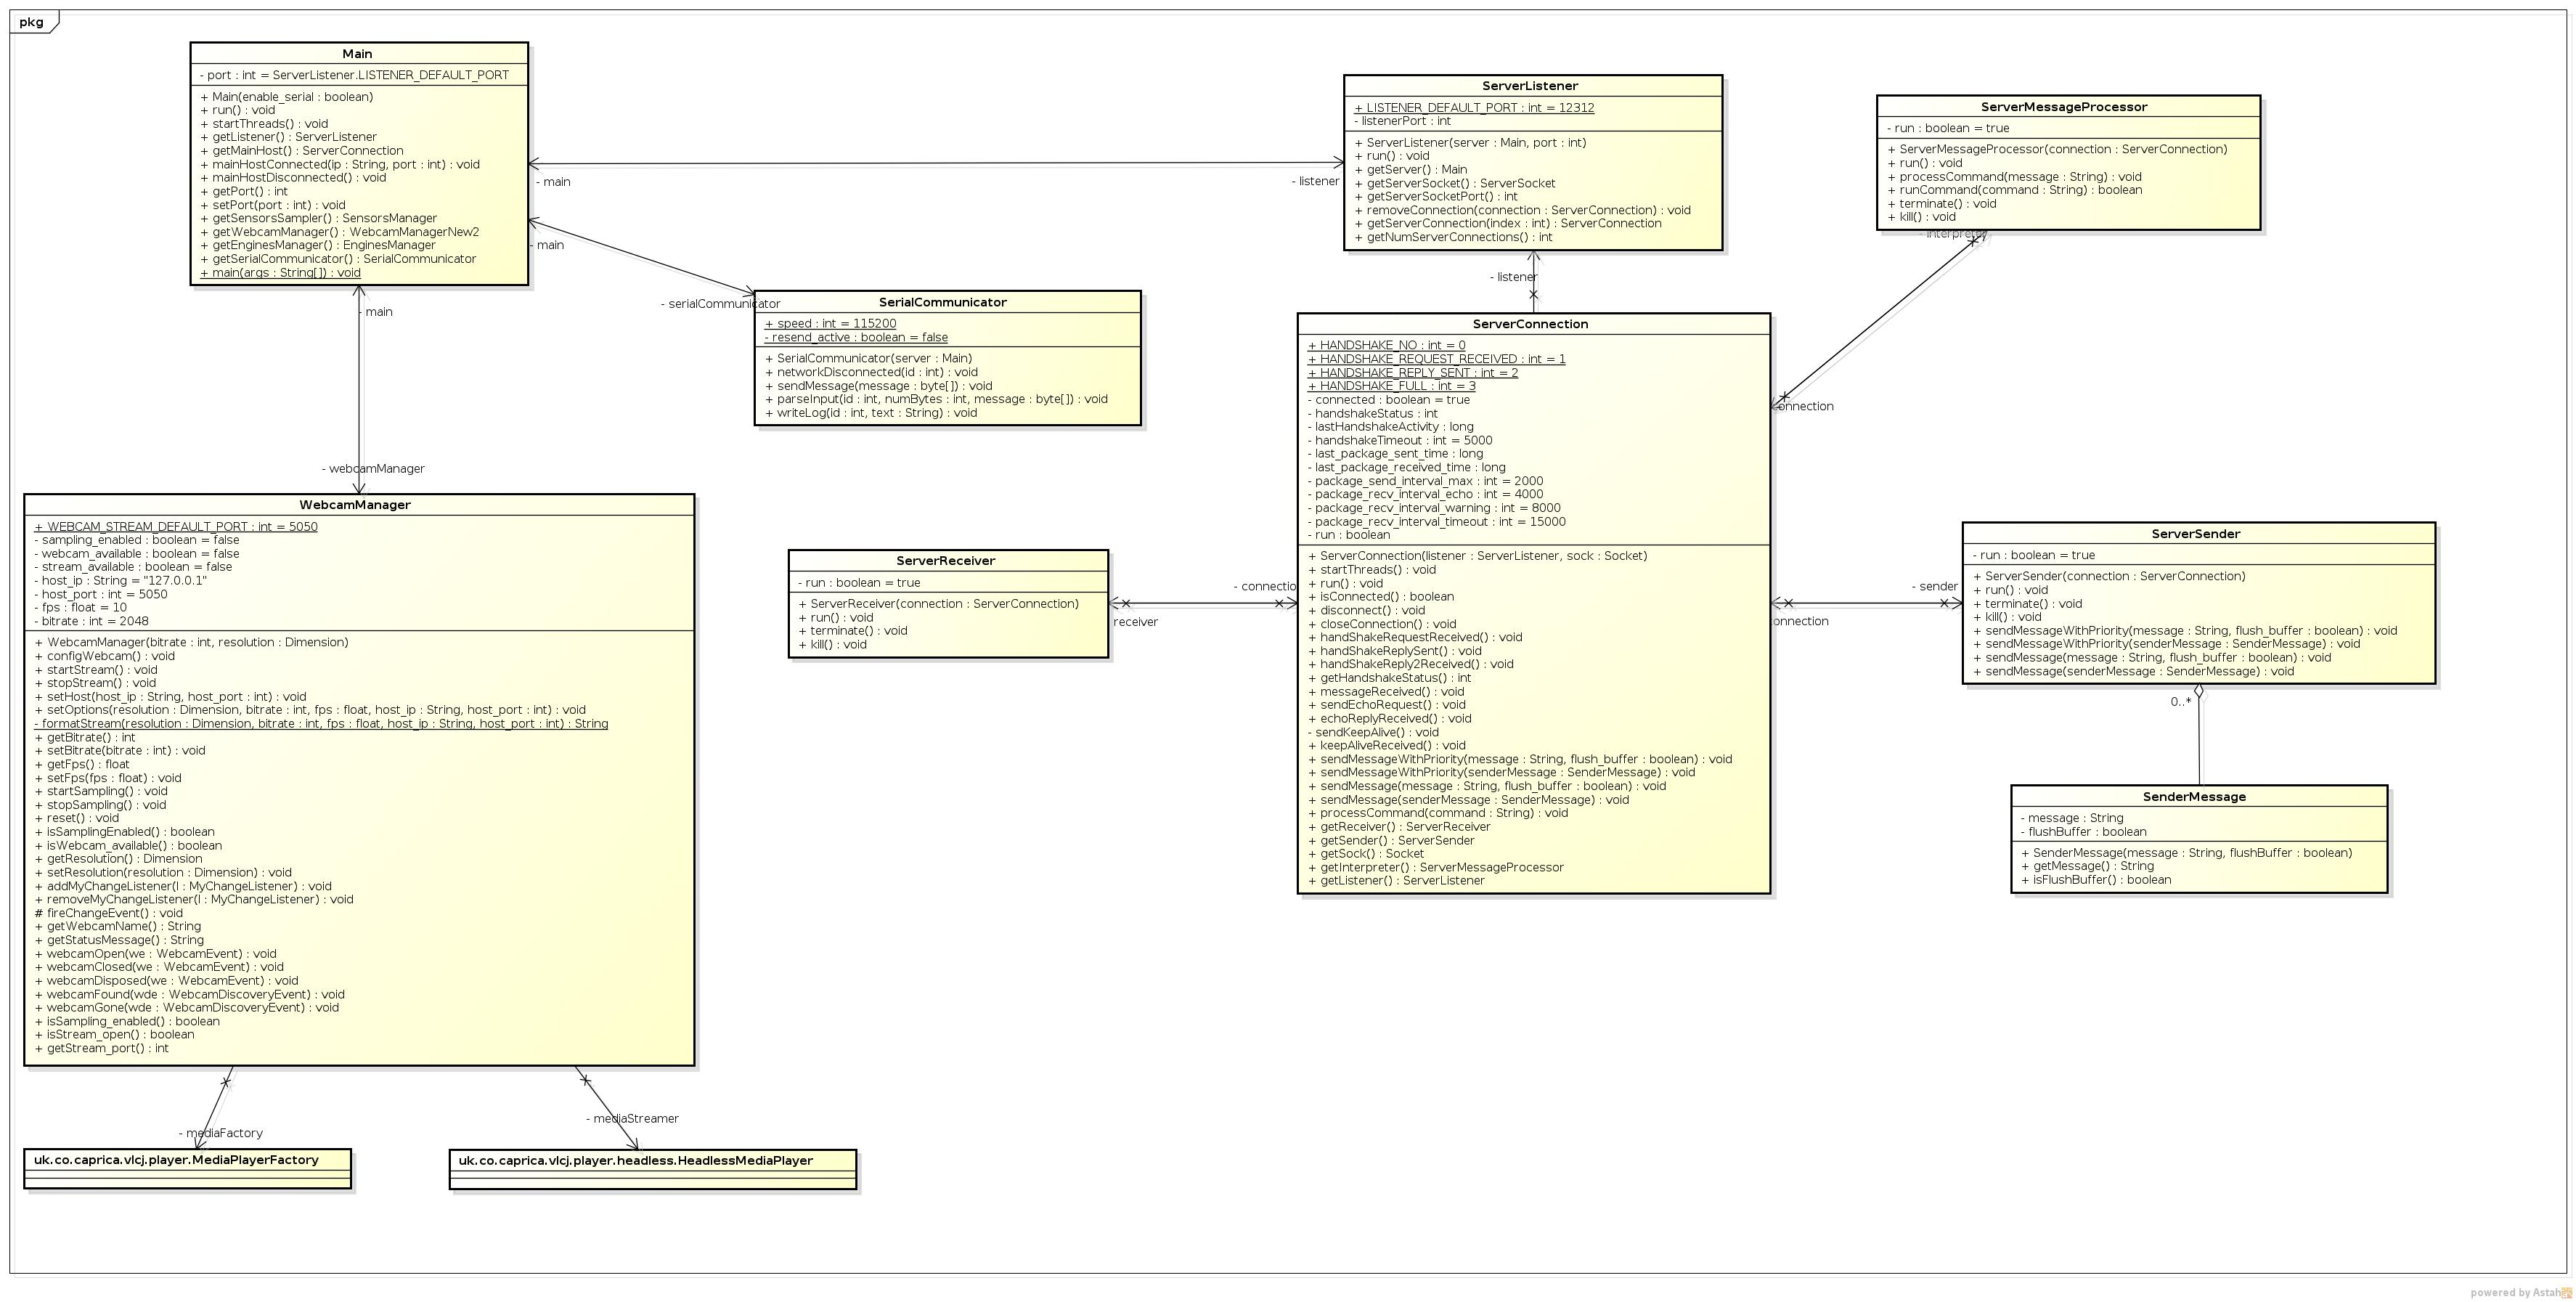
\includegraphics[width=\textwidth]{./figuras/sistEmbarcado/class_sistEmbarcado.jpg}
  \caption{Diagrama de classes do sistema embarcado (placa TS-7260).}
  \label{fig:diagrama_classes_sist_embarcado}
\end{figure}



%\subsection{Descrição das classes do sistema embarcado (TS-7260)}

\begin{table}[H]
  \centering
  \caption{Descrição das classes do sistema embarcado (placa TS-7260)}
  \begin{tabular}{p{6cm}p{8cm}}
    \toprule
    \textbf{Classe} & \textbf{Descrição} \\ 
    \midrule
   Main & Classe principal do robô. \\ \hline
   SensorsSampler & Thread responsável por requisitar amostras dos sensores da plca de baixo nível em intervalos de tempo previamente programados. \\ \hline
   ServerMessageProcessor & Thread responsável por realizar o processamento de mensagens recebidas de um host de conexão. \\ \hline
   ServerListener & Thread responsável por escutar requisições de conexão. \\ \hline
   ServerSender & Thread responsável por enviar mensagens ao host de uma conexão. \\ \hline
   SenderMessage & Contém uma mensagem que pode ser enviada por um Sender. \\ \hline
   ServerReceiver & Thread responsável por receber mensagens de um host de uma conexão. \\ \hline
   SerialCommunicator & Responsável por gerenciar a comunicação via porta serial entre a TS-7260 e a LPC2103.\\ \hline
   WebcamManager & Responsável por gerenciar a abertura e o fechamento da stream de imagens da webcam, além de configurar opções como resolução e taxa de frames. \\
   \bottomrule
  \end{tabular}%
  \label{tab:classes_ts}%
\end{table}%

\section{Cronograma original versus executado}
O cronograma original (Anexo D), foi executado conforme o esperado. Devido à antecipação de certas tarefas, eventuais atrasos ficaram dentro do planejado. Os deliverables foram entregues dentro do prazos estipulados.

\section{Orçamento original versus executado}
Como pode ser visto no orçamento em anexo, o custo total do projeto ficou em 899 reais, o que ultrapassou a inicial máxima em cerca de 18,9\%. Isso se deu, principalmente devido à ocorrência do risco de ``Taxação dos componentes comprados no exterior'', o que elevou signif